\documentclass{article}
\usepackage[utf8]{inputenc}
\usepackage{amsmath}
\usepackage{amssymb}
\usepackage[table]{xcolor}
\usepackage[a4paper, portrait, margin=0.95in]{geometry}
\usepackage{fancyhdr}
\usepackage{indentfirst}
\usepackage{ragged2e}
\pagestyle{fancy}
\usepackage{xcolor}
\usepackage{setspace}
\usepackage{tabularx}
\usepackage{graphicx}
\usepackage{subcaption}
\usepackage[export]{adjustbox}
\usepackage{array}
\usepackage{float}
\graphicspath{ {./images/} }
\lhead{SACAT Design Report}
\rhead{Team 10}

\usepackage{biblatex}
\addbibresource{ref.bib}


\begin{document}
% \setstretch{0.92}


\begin{titlepage}
    \begin{center}
        \vspace*{1cm}
            
        \LARGE
        \textbf{ENGF0002}\\
        \vspace{0.3cm}
        \textbf{Scenario 1}\\
        \vspace{0.3cm}
        \textbf{Design Report}\\
        \vspace{2cm}
        \huge
        \textbf{SACAT} \\
        \LARGE
        \vspace{0.3cm}
        \textbf{Sorting Algorithm Complexity Analysis Tool}\\
        \vspace{0.3cm}
        \vspace{1.0cm}
        \textbf{Team 10}\\
        \vspace{5cm}
        \textbf{Authors \& Student Numbers:}\\
        \vspace{0.3cm}
        \begin{center}
            \begin{tabular}{ c c }
                Andrzej Szablewski & 20016059 \\
                Tim Widmayer & 20006018 \\
                Szymon Duchniewicz & 20019971 \\
                Bartosz Grabek & 20016589 \\
            \end{tabular}
        \end{center}
            
        \vspace{3.0cm}    
        \textbf{University College London\\}
        \vspace{0.3cm}
        2020/2021%should there be a more precise date?
            
    \end{center}
\end{titlepage}

\tableofcontents
\vspace{1cm}
\listoffigures

    
\newpage
    \section{Introduction}
        \subsection{Motivation}
            Understanding the complexity of algorithms is a challenging task, in particular for novice programmers. As algorithms get more sophisticated, it becomes more difficult to analyse them and more important to test them in various circumstances. Comparing different algorithms without proper analytic tools can be tedious and time-consuming. There is a variety of algorithm implementations for any given problem, each with its own strengths and limitations. Therefore, a detailed and accurate comparison between different implementations is crucial.\\
            
            The first-year UCL undergraduate CS course "COMP0005: Algorithms" \cite{comp0005} covers widely used algorithms that solve the problem of sorting. For some of these algorithms, e.g. "Merge Sort", it is difficult ~– if not impossible – to grasp their functionality intuitively from reading a description in pseudocode. In the lecture slides, the professor used animations to demonstrate them, greatly enhancing the students' understanding. Seeing elements being sorted in real time is a valuable tool in learning about these algorithms. Visualisation is of great importance for programmers, since it gives an insight into the practical steps that a sorting algorithm performs.\\
            
            This need for a better understanding of sorting sparked the development of SACAT, Sorting Algorithm Complexity Analysis Tool. By validating, analysing and visualising students' implementations of sorting algorithms, SACAT will help them to understand the differences between theoretical and practical complexity analyses and also improve their programming skills.
             
        \subsection{Aim} 
            The aim of this project is to provide a sorting algorithm analysis tool that can be used by anyone trying to analyse and visualise their sorting algorithm implementation in Python code. The main features include:
            \begin{itemize}
            \item Validating the user's implementation of a sorting algorithm
            \item Empirical testing on random, semi-random and predefined data sets of the algorithm
                \begin{itemize}
                    \item time complexity through timing and counting the number of operations,
                    \item space complexity by recording memory allocation
                \end{itemize}
            \item Regression analysis and curve fitting to estimate the algorithm's big Oh and big Theta time and space complexity.
            \item Visualisation tools; in particular, plots showing the algorithm performance and bar charts showing the algorithm execution in real time.
            \end{itemize}

    \section{Application Design}
        \subsection{Program structure}
            The program will have a MVC (Model View Controller) architecture. The core logic is encapsulated in the Model, the GUI (Graphical User Interface) will be a part of the View and the Controller will regulate the communication between the two. This will allow easy addition of other views in the future, enabling a smooth migration of the entire program to a web or mobile app. \\
        
        \subsection{Resources}
            The program will be written in Python3, making use of the following additional libraries and modules:
            \begin{itemize}
                \item \verb|random| \textit{(built-in)} - Used for generating randomised tests to run on the input algorithm.
                \item \verb|math| \textit{(built-in)} - Used for performing advanced mathematical operations on test data and others.
                \item \verb|time| \textit{(built-in)} - Used for timing each test (to calculate time complexity) as well as to limit how long each test can run.
                \item \verb|tracemalloc| \textit{(built-in)} - Used for tracing the number of memory allocations and its usage.
                \item \verb|ast| \textit{(built-in)} - Used for building a custom profiler and adjusting parser.
                \item \verb|matplotlib| - Used for plotting the results of testing the input algorithm and the results of analysing that data. Used for animating graphs with the matplotlib.animation submodule.
                \item \verb|sklearn| - Used for analysing the data from the tests on the input algorithm. This module has built-in models for calculating Linear regression.
                \item \verb|numpy| - Used for manipulating test data and reorganising it.
                \item \verb|pyqt5| – Used for the GUI
        % other libs?
            \end{itemize}
            % What libraries we r using, (builtin random, matplotlib, etc), what language, what code structure Simon
    
        \subsection{GUI}
            The first version of the application will be a desktop app. One of the project deliverables is to develop a graphical user interface designed to make the interaction between the user and the Core simple and intuitive. The GUI is going to be implemented using PyQt5 (amongst other QT tools) and will be most likely a temporary shell of the app. Future plans include building a web application based on the Core (see section \ref{futureFeatures}) \\
            
            The interface will comprise of four main components:
            \begin {itemize}
                \item A text editor, in which the user will input their implementation either by typing it in or opening an existing one from an external file.
                \item A settings component, where the user will be able to specify the parameters of algorithm analysis such as $t_{max}$, $T_{max}$ and choose which testing and analytic methods to use.
                \item A visualisation segment containing interactive complexity graphs for time and space as well as the bar charts reflecting the behaviour of the sorting implementation.
                \item An information tool responsible for showing all the essential information at each stage of the analysis, including error messages, successful tests and fit results.
            \end {itemize}
            
            The GUI will also provide options for saving the code and the results of analyses, such that multiple implementations can be benchmarked against different factors. This will be achieved by allowing the user to name their implementation, making its results distinguishable from others. Then each analysis can be visualised distinctly on the plot graphs (for instance by using a specific color and updating the legend).
            
            \begin{figure}[H]
                \centering
                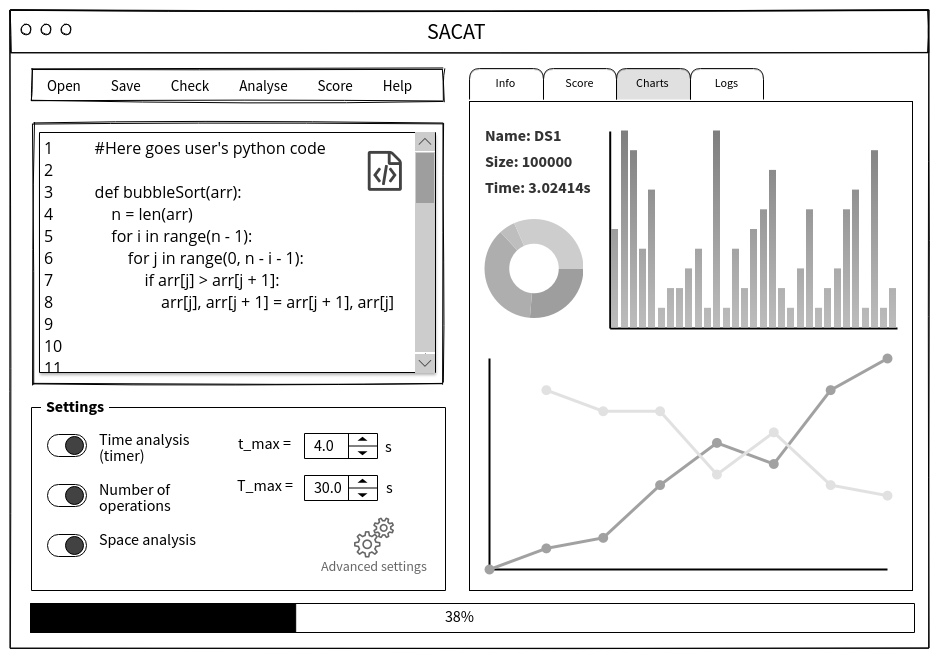
\includegraphics[scale=0.40]{images/gui.png}
                \caption{GUI Overview}
            \end{figure}
            
    \section{Methodology of Analysis}
            
            The model will estimate an algorithm time and space complexity based on data that is gathered during run-time. In the data gathering process, the program runs \textit{groups of tests} on the user's algorithm, each test producing a running cost (in terms of time, operations and memory) related to an input list type and length. After collecting all necessary data, they are analysed and used to estimate the complexity.
            
            \subsection{Time complexity based on time} \label{timeBasedComplx}
                One way of estimating the algorithm time complexity is to measure its \textit{time of execution} for different input lists. A downside of this approach is that it may not provide very precise results. Even on the same machine, results produced by running the same test twice may vary because of interruptions caused by other processes running simultaneously. The resulting noise may negatively affect the user's ability to distinguish between the performance of different algorithms, which would defeat the purpose of this tool to some extent.\\
                
                Nonetheless, estimating an algorithm's time complexity based on time plays a significant role in our design. The program is supposed to be a learning tool for a student. Therefore, including multiple ways of measuring performance can contribute to the student's understanding of algorithmic complexity. Crucially, this demonstrates the difference between the theoretical and real performance of algorithms.
            
            
            \subsection{Time complexity based on operation count} \label{nooBasedComplx}
                The most common definition of time complexity is the \textit{number of operations} that an algorithm performs. The operation count is independent of other processes running on the machine, which makes it a more precise measurement method of time complexity than execution time. Furthermore, it is independent of the CPU and memory of the device running the algorithm. \\
                
                To count operations, the user defined algorithm is firstly modified by an \textit{adjusting parser}, which adds the code necessary for the analysis. A custom-built profiler groups operations by type (e.g. comparisons, assignments) and measures precisely how many times each operation type is performed. The profiler will recognise which lines in the user defined sorting algorithm contain operations affecting the time complexity and will be able to measure their impact during run-time.

            
            \subsection{Space complexity}
                Calculating the space complexity will be based on a similar process as the one described for the calculating the time complexity. To estimate the space complexity usage, peak memory usage will be recorded for each corresponding list length. Then, all gathered data will be passed to the data analysis module. 

\newpage
    \section{Core Functionality} \label{corefunc}
        The model consists of several stages. In the \textit{Preliminary testing} stage, the user defined algorithm is tested for exceptions and correct functioning (e.g. sorting lists correctly). If the algorithm passes this stage, the \textit{data gathering} process begins which runs the algorithm multiple times. While performing sorting, it is monitored by different run environments. After gathering an appropriate amount of data, the \textit{data analysis} algorithms start and output their estimations. The general process is presented in Figure \ref{fig:core structure}.
            
        \begin{figure}[H]
        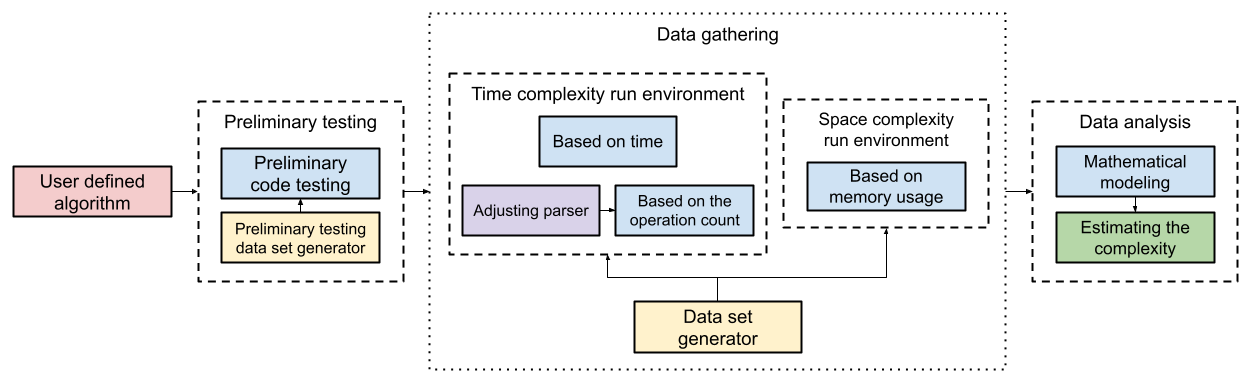
\includegraphics[width=1.0\textwidth]{model_diagram.png}
        \caption{Core general structure}
        \label{fig:core structure}
        \end{figure}
    
        \subsection{User input}
            An algorithm that the user inputs must obey several rules to be correctly analysed by the program:
            \begin{itemize}
                \item The algorithm must be executed through a function called \verb|sort|, which takes a python list called \verb|array| as its only parameter. This does not prevent the algorithm from having more than one function, since \verb|sort| can call auxiliary functions.
                \item The algorithm must not rely on external libraries or imports from local files.
                \item The algorithm cannot modify or access any files or system settings. Besides, any such attempt will be blocked by the run environments.
            \end{itemize}
        
        \subsection{Preliminary Testing}
            Before testing the complexity of the user defined sorting algorithm, the system must validate that the algorithm executes without errors and sorts lists properly. If the code throws exceptions, they must be handled by the program and the user should be warned that the code does not run properly. The first step here should be to run the user's code on a randomly generated list of 100 integers.\\
            
            If there are no exceptions, the output list must be validated. This can be achieved by looping through the entire list and checking whether the first of two consecutive elements is equal or smaller to the second one. After this initial validation, the program will test the following corner cases:
            \begin{itemize}
                \item An empty list, \verb|[]|
                \item A 1-element list, e.g. \verb|[1]|
                \item A sorted list, e.g. \verb|[1, 2, 3, ..., 100]|
                \item A sorted list in reversed order, e.g. \verb|[100, 99, 98, ...,1]|
                \item A list containing equal elements, e.g. \verb|[1, 1, 1, ..., 1]|
                \item A list of odd length, e.g. \verb|[2,3,8,2,9]| and even length, e.g. \verb|[2,9,1,3,9,4]|
            \end{itemize}
            When these tests are passed – i.e. no exceptions are raised – the algorithm is ready to be analysed for time and space complexity.
            
        \subsection{Data gathering}
            Data gathering plays a key role in estimating the complexity of an algorithm. The mathematical models described in section \ref{dataAnalysis} require a sufficient number of data points to attain statistically significant results.
            
            \subsubsection{Time limits}
                Since the time that it takes an algorithm to sort a list can get arbitrarily long, it is important to run each test within an environment that keeps the time elapsed since the start of a test. If this time passes a certain threshold $t_{max}$, the test should be aborted and with it all tests that would have taken place in the future. The faster the algorithm, the more data could be collected within $t_{max}$, increasing the analysis' precision. This threshold value is modifiable by the user in the program settings.\\
                
                Limiting the total number of tests to be performed would not be effective because sort algorithms can vary significantly in performance. Instead, the user can specify an upper bound on the time spent on all tests, $T_{max}$. This time limit will be distributed equally across all \textit{groups of tests}.\\
            
            \subsubsection{Groups of tests} \label{testingDataSets}
                The length of the input list is not the only factor affecting the time complexity of a sort algorithm. Other factors that should be considered are, for example, the number of duplicates in the list or whether the list is already sorted. Therefore, \textit{groups of tests} are specified and run separately. This enables the program to provide a more nuanced analysis, showing not only the estimated \textit{average} time complexity, Big Theta, (i.e. performance on randomly generated lists), but also the \textit{worst case} time complexity, Big Oh.\\
                
                \noindent The following groups of tests are run:
                \begin{enumerate}
                    \item Random lists – average case: lists consisting of elements randomly generated within a relatively wide range, such that it is unlikely that they contain many duplicates.
                    \item Duplicate lists – worst-case: lists consisting of elements randomly generated within a relatively tight range, such that they contain many duplicates. For some algorithms this may result in the worst time complexity.
                    \item Sorted lists – worst-case. For some algorithms this may result in the worst.
                    \item Reverse sorted lists – worst-case: sorted lists in reversed order. For some algorithms this may result in the worst time complexity.
                \end{enumerate}
                
                 The average case will be estimated using data from running a \textit{Random lists} group of tests, and the worst case will be estimated by taking the worst calculated complexity using data from all groups of tests.\\
                
                \noindent For each group of tests, lists of increasing length are generated by the program until time reserved for this group has elapsed. If needed, Python's \verb|random| module is used to generate random numbers. The length of the lists in a group of tests will be increased exponentially using the formula: $$S_i = 10^{0.1i},$$ where $i$ is the number of test beginning with 0 and $S_i$ is the number of elements in the list.\\
                
                Although by default elements will be positive integers, user will be able to choose the type of elements in input lists from:
                \begin{itemize}
                    \item positive integers,
                    \item negative integers,
                    \item integers,
                    \item doubles.
                \end{itemize} 
                
        \subsection{Data analysis} \label{dataAnalysis}
                As mentioned in the previous sections, the groups of data to be analysed are:
                \begin{itemize}
                    \item time of execution,
                    \item operations count,
                    \item peak memory allocated.
                \end{itemize}
                These values (dependent variables) would be compared against lists of unsorted data with varying length (the independent variable).  Each independent variable is plotted in several encodings against the input length:
                \begin{itemize}
                    \item Polynomial: $y = x, y = x^2, y=x^3$,
                    \item Linearithmic: $y=x \log x$,
                    \item Exponential: $y=2^x$,
                \end{itemize}
                where $x$ is substituted with the independent variable (length of a list), and the resulting $y$ plotted against it.
                The aim of these plots is to perform linear regression using the Ordinary Least Squares method – or different methods such as curve fitting or polynomial interpolation – on the data with a model supplied by the \verb|sklearn| library. Then, the resulting correlation coefficients are used to estimate the tested algorithm's  complexity class. The plots with the highest coefficients indicate the most likely complexities and they will be displayed to the user.\\

        \subsection{Example Analyses}
            \subsubsection{Mergesort}
            This example shows how the method described in Section \ref{dataAnalysis} would estimate Big Oh complexity of mergesort. The graph of time versus list length (Figure \ref{fig: merge}) shows the gathered test data. The closest fit based on the correlation coefficients below is $O(n\,log \,n)$. \\
            
            \noindent
            \begin{minipage}{0.45\textwidth}
            \centering
            \begin{tabular}{|l|c|}
                \hline
                Methods used & Ordinary least Squares \\
                \hline
                Values measured & time \\
                \hline
                Testing lists lengths &  from 1 to 1 000 000\\
                \hline
                Number of readings & 50 \\
                \hline
                \end{tabular}
                
            \vspace{1cm}
            \begin{tabular}{|l|c|}
                \hline
                $O(n)$ fit & 0.9980142465341569 \\
                \hline
                $\mathbf{O(n\,log\,n)}$ \textbf{fit} & \textbf{0.999183245476026} \\
                \hline
                $O(n^2)$ fit & 0.9512071398181208 \\
                \hline
                
            \end{tabular}

            \end{minipage}
            \begin{minipage}{0.6\textwidth}
            \begin{figure}[H]
                    % \centering
                    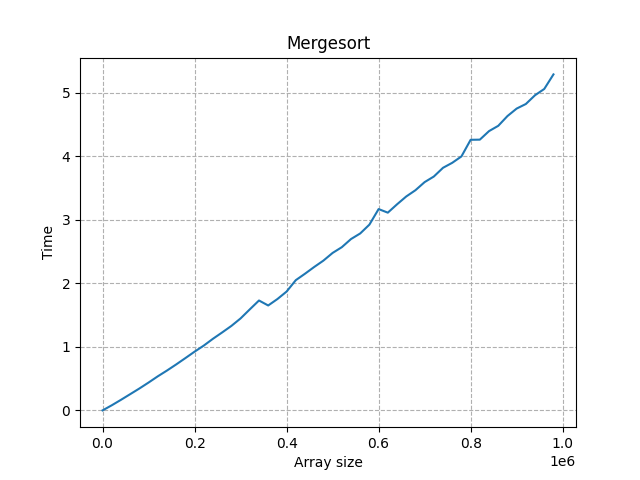
\includegraphics[scale=0.58, right]{images/mergesort_grid_1mil_50readingsv2.png}
                    \caption{Mergesort data}
                    \label{fig: merge}
            \end{figure}
            \end{minipage}

\newpage
            \subsubsection{Heapsort}
             This example shows how the method described in Section \ref{dataAnalysis} would estimate Big Oh complexity of heapsort. The graph of time versus list length (Figure \ref{fig: heapsort}) shows the gathered test data. The closest fit based on the correlation coefficients below is $O(n\,log \,n)$.\\
            \noindent
            \begin{minipage}{0.45\textwidth}
            \centering
            \begin{tabular}{|l|c|}
                \hline
                Methods used & Ordinary least Squares \\
                \hline
                Values measured & time \\
                \hline
                Testing lists lengths &  from 1 to 1 000 000\\
                \hline
                Number of readings & 50 \\
                \hline
                \end{tabular}
                
            \vspace{1cm}
            \begin{tabular}{|l|c|}
                \hline
                $O(n)$ fit & 0.996427980316863 \\
                \hline
                $\mathbf{O(n\,log\,n)}$ \textbf{fit} & \textbf{0.998390222043668} \\
                \hline
                $O(n^2)$ fit: & 0.9570196636456305 \\
                \hline
                
            \end{tabular}

            \end{minipage}
            \begin{minipage}{0.6\textwidth}
            \begin{figure}[H]
                    % \centering
                    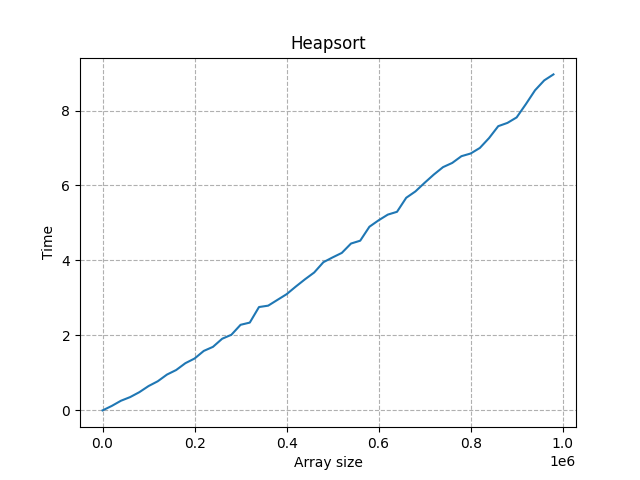
\includegraphics[scale=0.58, right]{images/heapsort_grid_1mil_50readingsv2.png}
                    \caption{Heapsort data}
                    \label{fig: heapsort}
            \end{figure}
            \end{minipage}

            \subsubsection{Bubblesort}
                This example shows how the method described in Section \ref{dataAnalysis} would estimate Big Oh complexity of bubblesort. The graphs of time versus list length (Figure \ref{fig: time based bubble}) as well as operations versus list length (Figure \ref{fig: op count based bubble} show the gathered test data. The closest fit based on the correlation coefficients below is $O(n^2)$ for both time and operations count analyses. Additionally, the graph in Figure \ref{fig: op count based bubble} is noticeably smoother than the one in Figure \ref{fig: time based bubble}. This demonstrates that tests based on counting operations generate significantly less noise compared to tests based on timing.\\
        \begin{center}

            \begin{tabular}{|l|c|}
                \hline
                Methods used & Ordinary least Squares \\
                \hline
                Values measured & time \& operations count \\
                \hline
                Testing lists lengths &  from 1 to 4 000\\
                \hline
                Number of readings & 50 \\
                \hline
            \end{tabular}
        \end{center}
        
            \noindent
            \begin{minipage}{0.5\textwidth}
            \centering
            \begin{tabular}{|l|c|}
                \hline
                $O(n)$ fit (time) & 0.9330138172471819 \\
                \hline
                $O(n\,log\,n)$ fit (time) & 0.9511589788294077 \\
                \hline
                $\mathbf{O(n^2)}$ \textbf{fit (time)} & \textbf{0.9988990483424111} \\
                \hline
            \end{tabular}
            \end{minipage}            
            \begin{minipage}{0.5\textwidth}
            \centering
            \begin{tabular}{|l|c|}
                \hline
                $O(n)$ fit (op.) & 0.9352182627367351 \\
                \hline
                $O(n\,log\,n)$ fit (op.) & 0.9532947615243036 \\
                \hline
                $\mathbf{O(n^2)}$ \textbf{fit (op.)} & \textbf{0.9999999960611927}\\
                \hline
                
            \end{tabular}
            \end{minipage}
            
            \begin{figure}[H]
                \begin{subfigure}{.5\textwidth}
                \centering
                    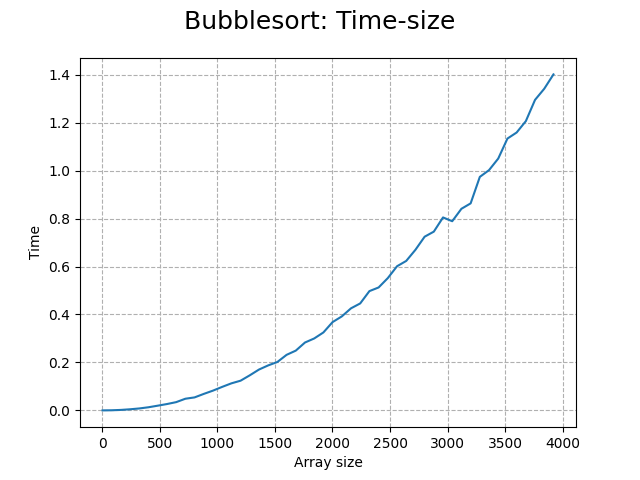
\includegraphics[scale=0.45]{images/bubblesort_grid_4k_50readings_time.png}
                    \caption{Time based}
                    \label{fig: time based bubble}
                \end{subfigure}
                \begin{subfigure}{.5\textwidth}
                \centering
                    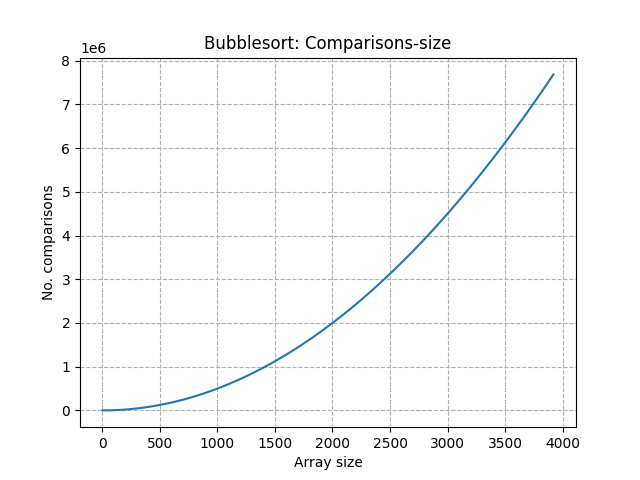
\includegraphics[scale=0.45]{images/bubblesort_grid_4k_50readings_comparisons.png}
                    \caption{Operations count based}
                    \label{fig: op count based bubble}
                \end{subfigure}
                \caption{Bubblesort data}
            \end{figure}


    \section{Possible Future Improvements} \label {futureFeatures}
        Due to time limitations, not all of the project possible features can be implemented, yet there is a number of possible future improvements to be developed. These include:
        \begin{itemize}
            \item Web deployment of the app to make it accessible to a wider audience.
            \item Analysis of algorithms based on user-defined data sets.
            \item A scoring feature to introduce competitiveness, which could motivate users to do more research on algorithms and experiment with the tool.
            \item Analysing algorithms operating on other data structures (not Python lists), e.g. trees, linked lists.
            \item Analysing algorithms that solve other problems, e.g. search.
        \end{itemize}

\newpage

    % \section{Bibliography}
    % \begin{itemize}
    %     \item UCL Computer Science "COMP0005: Algorithms" Lectures by Module Lead, Prof. Licia Capra 
    %     \item 2011. Algorithms / Robert Sedgewick and Kevin Wayne. 4th ed., Upper Saddle River, N.J. ; London: Addison-Wesley Professional.
    % \end{itemize}
    
\nocite{*}
\printbibliography
\end{document}